\chapter{Равносильность, рациональные и иррациональные задачи}\label{chap:exam-rational}\markright{Глава 13}
\section{Область допустимых значений и логика решения}
Решать уравнение — значит найти все допустимые значения неизвестных, для которых оно верно. В этой главе неизвестные действительные. Сначала устанавливаем, где исходные выражения определены, затем обосновываем преобразования и в конце записываем множество решений.
\begin{definition}\term{Равносильные условия} (equivalent conditions) на множестве \(D\) имеют одно и то же множество решений в \(D\); пишут \(A\Longleftrightarrow B\).\end{definition}
\begin{definition}Условие \(B\) называется \term{следствием} (logical consequence) условия \(A\), если каждое решение \(A\) удовлетворяет \(B\); пишут \(A\Longrightarrow B\). Обратное утверждение может быть неверным.\end{definition}
\begin{definition}\term{Система} (system) требует одновременного выполнения всех входящих в неё условий.\end{definition}
\begin{definition}\term{Совокупность} (disjunction of conditions) требует выполнения хотя бы одного из входящих в неё условий.\end{definition}
Множество решений системы есть пересечение, совокупности — объединение множеств решений её условий.
\par\addvspace{2pt}\begin{lrbox}{\CatFlowBox}\begin{minipage}[t]{\linewidth}
\setlength{\parskip}{2pt}\setlength{\columnsep}{4.5mm}\setlength{\intextsep}{0pt}
\begin{wrapfigure}[11]{r}{54mm}

\includegraphics[width=54mm,height=58mm,keepaspectratio]{images/unique/art-218.png}
\label{catflow:218}
\end{wrapfigure}
Решение начинается с записи исходных ограничений. Знаменатели не должны обращаться в нуль, а подкоренные выражения квадратных корней должны быть неотрицательными. После сокращения дроби эти ограничения продолжают действовать, даже если в новой записи запрещённая точка больше не видна. Полезно вести два списка: допустимые значения и кандидаты в решения. Равносильное преобразование сохраняет второй список точно; переход к следствию может его расширить. Тогда каждый оставшийся кандидат проверяют в исходном условии. Такой порядок особенно важен при нескольких действиях подряд: потерянное ограничение иногда обнаруживается только в самом конце, когда красивый короткий ответ уже кажется убедительным. Проверка возвращает нас к исходной задаче и связывает вычисления с определением решения.
\par\WFclear\end{minipage}\end{lrbox}%
\ifdim\dimexpr\ht\CatFlowBox+\dp\CatFlowBox\relax<58mm\dp\CatFlowBox=\dimexpr58mm-\ht\CatFlowBox\relax\fi%
\noindent\usebox{\CatFlowBox}\par\addvspace{2pt}
\begin{theorem}[Безопасные преобразования]
Пусть все выражения определены на \(D\). Прибавление одного выражения к обеим частям уравнения равносильно. Умножение обеих частей на \(H(x)\), нигде не равное нулю на \(D\), также равносильно. Для действительных \(F,G\)
\[
F=G\quad\Longleftrightarrow\quad
\begin{cases}F^2=G^2,\\FG\geq0.\end{cases}
\]
\end{theorem}
\begin{proof}Прибавление отменяется вычитанием; умножение на ненулевое число отменяется делением. Из \(F^2=G^2\) следует \((F-G)(F+G)=0\), поэтому \(F=G\) или \(F=-G\). Во втором случае \(FG=-F^2\geq0\) возможно лишь при \(F=G=0\). Обратное направление очевидно.\end{proof}
Деление на выражение с неизвестным без проверки его нулей может потерять решения. Например, \(x(x-2)=x\) равносильно \(x(x-3)=0\), откуда \(x=0\) или \(x=3\). Деление на \(x\) оставило бы только второй корень. Умножая неравенство на выражение неизвестного знака, отдельно разбирают положительный, отрицательный и нулевой случаи.
\begin{example}Решим \(\frac{x^2-4}{x-2}=4\). ОДЗ: \(x\ne2\). На ней уравнение равносильно \(x+2=4\), но единственный кандидат \(x=2\) запрещён. Решений нет. Равенство дроби и многочлена при допустимых значениях не разрешает расширять исходную ОДЗ.\end{example}

\section{Системы: подстановка и сложение}
В методе подстановки из одного уравнения выражают неизвестное и подставляют в остальные. Обратная подстановка обязательна: ответом системы с двумя неизвестными служат пары. В методе сложения одно уравнение заменяют его суммой с кратным другого, сохраняя само другое уравнение. Такая операция обратима вычитанием того же кратного. Если коэффициент, на который требуется делить, может быть нулём, сначала выделяют этот случай.
\begin{example}Из \(x+y=5\), \(xy=6\) получаем \(y=5-x\), затем \(x(5-x)=6\). Поэтому \((x-2)(x-3)=0\), и пары равны \((2,3)\), \((3,2)\). Оба порядка нужны. Для линейной системы \(2x+y=7\), \(x-y=2\) сложение даёт \(3x=9\); далее \(x=3,y=1\).\end{example}

\section{Факторизация и формулы Виета}
\begin{theorem}[Виет и обратное утверждение]
Если \(a\ne0\), то числа \(r,s\), включая возможность \(r=s\), являются корнями \(ax^2+bx+c=0\) с учётом кратности тогда и только тогда, когда
\[
r+s=-\frac ba,\qquad rs=\frac ca.
\]
В этом случае \(ax^2+bx+c=a(x-r)(x-s)\).
\end{theorem}
\begin{proof}Раскрытие скобок справа даёт \(ax^2-a(r+s)x+ars\); сравнение коэффициентов доказывает обе стороны. Если корни уже известны, разложение следует из формулы корней квадратного уравнения: \(r+s=-\frac ba\), \(rs=\frac{b^2-D}{4a^2}=\frac ca\).\end{proof}
Факторизацию ищут последовательно: общий множитель, формулы квадратов и кубов, группировка, затем подбор корня и деление на линейный множитель. Замена \(t=x^2\) требует \(t\geq0\): положительное \(t\) даёт два значения \(x\), нуль — одно, отрицательное — ни одного. Замена должна сопровождаться описанием всех обратных подстановок.

\section{Метод интервалов с учётом кратности}
\begin{definition}\term{Кратность нуля} (multiplicity of a zero) равна показателю \(m\) в разложении \(P(x)=(x-r)^mQ(x)\), где \(Q(r)\ne0\).\end{definition}
\begin{theorem}[Знак рационального произведения]
Пусть рациональная функция разложена на ненулевую константу и целые положительные степени линейных множителей числителя и знаменателя. Между соседними различными нулями этих множителей знак постоянен. При переходе через отмеченную точку знак меняется тогда и только тогда, когда разность кратностей её множителей в числителе и знаменателе нечётна. Общие множители можно сократить для вычисления знака, сохраняя исходные запреты.
\end{theorem}
\begin{proof}На промежутке каждый линейный множитель имеет постоянный знак. Через точку \(r\) меняют знак только множители \(x-r\); степень чётной кратности знак сохраняет, нечётной — меняет. Отношение знаков даёт правило разности кратностей. Исходная дробь в нуле знаменателя не определена даже после сокращения.\end{proof}
\par\addvspace{2pt}\begin{lrbox}{\CatFlowBox}\begin{minipage}[t]{\linewidth}
\setlength{\parskip}{2pt}\setlength{\columnsep}{4.5mm}\setlength{\intextsep}{0pt}
\begin{wrapfigure}[11]{l}{54mm}
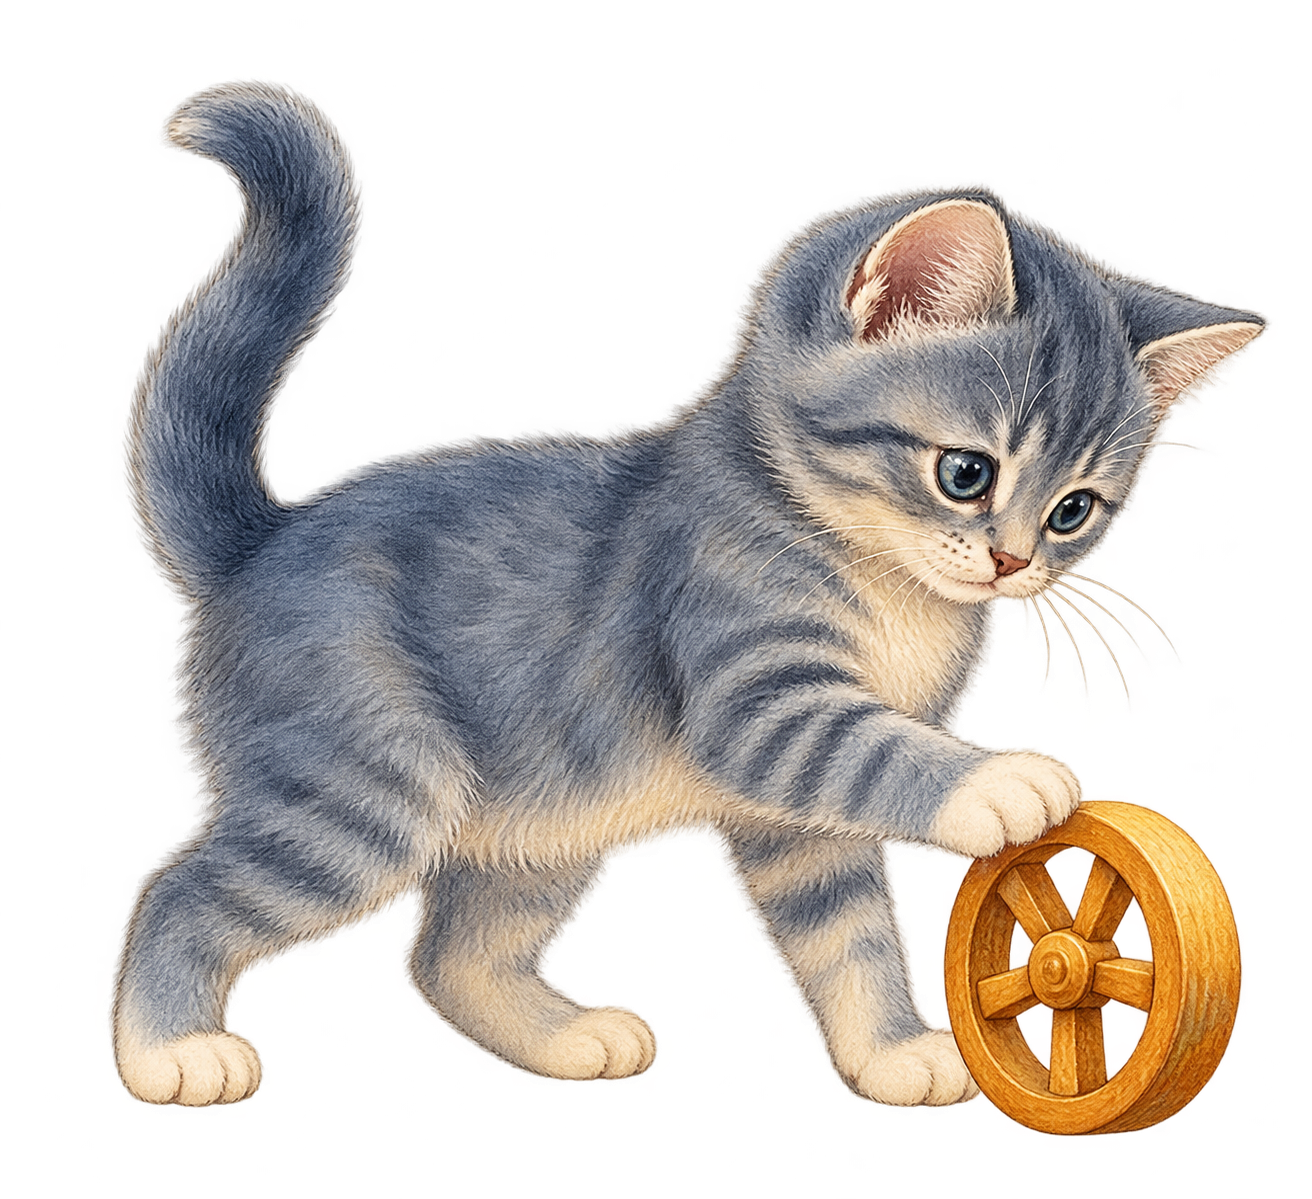
\includegraphics[width=54mm,height=58mm,keepaspectratio]{images/unique/art-219.png}
\label{catflow:219}
\end{wrapfigure}
Проверка знака начинается с крайнего правого промежутка. Там все линейные множители вида \(x-r\) положительны, поэтому достаточно знака вынесенной константы. Затем можно двигаться влево, меняя знак только на точках нечётной общей кратности. Однако таблица знаков ещё не является ответом. Для строгого неравенства нули числителя исключают; для нестрогого включают, если сама дробь там определена. Запрещённые точки никогда не включают. Если числитель имеет чётную кратность, отдельный нуль способен попасть в ответ даже тогда, когда соседние промежутки не подходят. Поэтому в записи результата полезно явно проверить каждую отмеченную точку, а не только закрашенные промежутки между ними.
\par\WFclear\end{minipage}\end{lrbox}%
\ifdim\dimexpr\ht\CatFlowBox+\dp\CatFlowBox\relax<58mm\dp\CatFlowBox=\dimexpr58mm-\ht\CatFlowBox\relax\fi%
\noindent\usebox{\CatFlowBox}\par\addvspace{2pt}
\begin{example}Решим \(\frac{(x-2)^2}{x+1}\leq0\). ОДЗ: \(x\ne-1\). При \(x<-1\) дробь отрицательна. При \(x>-1\) она положительна, кроме нуля \(x=2\). В этой точке нестрогое неравенство верно. Ответ: \(( -\infty;-1)\cup\{2\}\). Кратный нуль здесь даёт отдельную точку, а не границу подходящего интервала.\end{example}

\section{Иррациональные уравнения и неравенства}
\begin{definition}\term{Иррациональное уравнение} (radical equation) содержит неизвестное под знаком корня. При работе с квадратным корнем всегда используется его неотрицательное значение.\end{definition}
\begin{theorem}[Устранение квадратного корня]
Для действительных выражений \(F,G\) верны равносильности
\[
\sqrt F=G\ \Longleftrightarrow\ F=G^2,\ G\geq0;
\]
\[
\sqrt F\leq G\ \Longleftrightarrow\ F\geq0,\ G\geq0,\ F\leq G^2;
\]
\[
\sqrt F>G\ \Longleftrightarrow\ F\geq0\ \text{и}\
\bigl(G<0\ \text{или}\ (G\geq0\ \text{и}\ F>G^2)\bigr).
\]
Для \(\sqrt F<G\) нужны \(F\geq0,G>0,F<G^2\).
\end{theorem}
\begin{proof}Квадратный корень неотрицателен. На неотрицательных числах возведение в квадрат строго возрастает, поскольку \(v^2-u^2=(v-u)(v+u)>0\) при \(0\leq u<v\). Поэтому сравнение с неотрицательной правой частью можно возвести в квадрат; отрицательная правая часть разбирается непосредственно. В равенстве \(F=G^2\) условие \(F\geq0\) уже выполнено.\end{proof}
\begin{example}Решим \(\sqrt{5-x}>x-1\). ОДЗ: \(x\leq5\). При \(x<1\) правая часть отрицательна и неравенство верно. При \(1\leq x\leq5\) можно возвести в квадрат: \(5-x>(x-1)^2\), то есть \(x^2-x-4<0\). На этой ветви получаем \(1\leq x<\frac{1+\sqrt{17}}2\). Объединяя ветви, находим \(x<\frac{1+\sqrt{17}}2\).\end{example}

\begin{theorem}[Корни высших степеней]
При нечётном натуральном \(n\) функция \(t\mapsto t^n\) строго возрастает на всей прямой. Поэтому \(\sqrt[n]{F}=G\) равносильно \(F=G^n\), а сравнение \(\sqrt[n]{F}\leq G\) — сравнению \(F\leq G^n\), без ограничений на знаки \(F,G\). Для чётного \(n\geq2\) арифметический корень требует \(F\geq0\), а все правила для квадратного корня сохраняются с заменой \(G^2\) на \(G^n\).
\end{theorem}
\begin{proof}При \(0\leq u<v\) разность \(v^n-u^n=(v-u)(v^{n-1}+v^{n-2}u+\cdots+u^{n-1})\) положительна. Для нечётного \(n\) отражение относительно нуля даёт возрастание также на отрицательной полуоси; сравнение чисел разных знаков очевидно. Для чётного \(n\) применяем доказанное возрастание лишь к неотрицательным значениям арифметического корня и правой части, предварительно разбирая знак последней.\end{proof}
\begin{example}Решим \(\sqrt[3]{x+6}=x\). Нечётная степень сохраняет равносильность без ограничений на знак: \(x+6=x^3\). Получаем \((x-2)(x^2+2x+3)=0\). Второй множитель равен \((x+1)^2+2>0\), поэтому единственный корень \(x=2\).\end{example}

\section{Модуль и разбиение на случаи}
\begin{theorem}[Раскрытие модуля]
Для \(c\geq0\) условие \(|F|\leq c\) равносильно \(-c\leq F\leq c\), а \(|F|\geq c\) — совокупности \(F\leq-c\) или \(F\geq c\). Если \(c>0\), аналогично действуют строгие знаки. При \(c=0\) условие \(|F|<0\) невозможно, а \(|F|>0\) означает \(F\ne0\).
\end{theorem}
\par\addvspace{2pt}\begin{lrbox}{\CatFlowBox}\begin{minipage}[t]{\linewidth}
\setlength{\parskip}{2pt}\setlength{\columnsep}{4.5mm}\setlength{\intextsep}{0pt}
\begin{wrapfigure}[11]{l}{54mm}

\includegraphics[width=54mm,height=58mm,keepaspectratio]{images/unique/art-221.png}
\label{catflow:221}
\end{wrapfigure}
\textit{Доказательство.} При \(F\geq0\) имеем \(|F|=F\), при \(F<0\) имеем \(|F|=-F\). Разбор этих двух случаев даёт все утверждения.\hfill\(\blacksquare\)
\par\WFclear\end{minipage}\end{lrbox}%
\ifdim\dimexpr\ht\CatFlowBox+\dp\CatFlowBox\relax<58mm\dp\CatFlowBox=\dimexpr58mm-\ht\CatFlowBox\relax\fi%
\noindent\usebox{\CatFlowBox}\par\addvspace{2pt}

Если справа стоит выражение \(G(x)\), сначала определяют его знак. При \(G<0\) условие \(|F|\leq G\) невозможно, а \(|F|>G\) верно всюду на ОДЗ. Несколько модулей удобно раскрывать на промежутках, границами которых являются нули всех подмодульных выражений.
\par\addvspace{2pt}\begin{lrbox}{\CatFlowBox}\begin{minipage}[t]{\linewidth}
\setlength{\parskip}{2pt}\setlength{\columnsep}{4.5mm}\setlength{\intextsep}{0pt}
\begin{wrapfigure}[10]{r}{54mm}
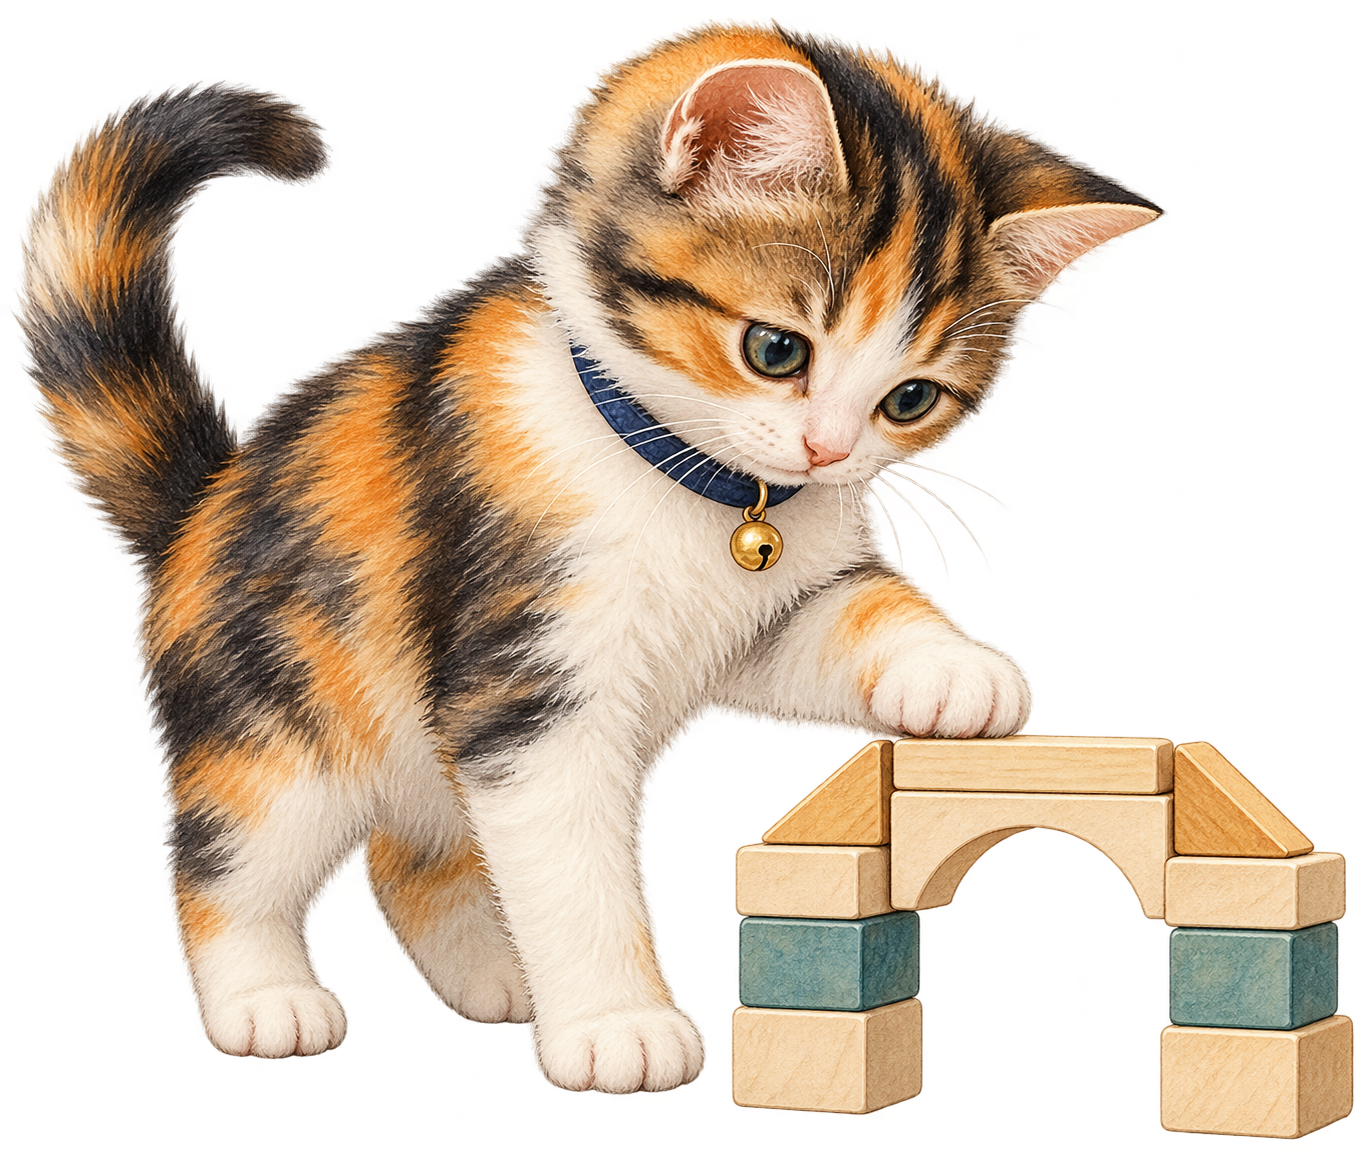
\includegraphics[width=54mm,height=58mm,keepaspectratio]{images/unique/art-220.png}
\label{catflow:220}
\end{wrapfigure}
Разбиение прямой на промежутки превращает задачу с модулями в несколько обычных уравнений. Границы выбирают по знакам выражений внутри модулей, а найденные корни оставляют только в том промежутке, где было получено соответствующее уравнение. Одну граничную точку иногда удобно рассмотреть отдельно, чтобы она не исчезла между двумя строгими случаями. После объединения одинаковые корни записывают один раз. Геометрический смысл расстояния помогает проверить результат: сумма расстояний до двух фиксированных точек постоянна между ними и возрастает при удалении наружу. Этот взгляд позволяет заранее оценить число корней, но окончательная запись всё равно должна содержать точные границы и проверенные значения.
\par\WFclear\end{minipage}\end{lrbox}%
\ifdim\dimexpr\ht\CatFlowBox+\dp\CatFlowBox\relax<58mm\dp\CatFlowBox=\dimexpr58mm-\ht\CatFlowBox\relax\fi%
\noindent\usebox{\CatFlowBox}\par\addvspace{2pt}
\begin{example}В \(|x-1|+|x-4|=5\) при \(x\leq1\) получаем \(5-2x=5\), откуда \(x=0\). При \(1\leq x\leq4\) сумма равна \(3\), поэтому решений нет. При \(x\geq4\) имеем \(2x-5=5\), откуда \(x=5\). Оба корня удовлетворяют своим ограничениям; ответ \(\{0,5\}\).\end{example}

\relax

\Needspace{7\baselineskip}\section*{Задачи}
\begingroup\setlength{\parskip}{1pt}
\noindent\begin{minipage}[t]{\linewidth}\textbf{13.1.} Найди ОДЗ выражения \(\dfrac{\sqrt{x-1}}{x^2-5x+6}\).\par\end{minipage}\par
\noindent\begin{minipage}[t]{\linewidth}\textbf{13.2.} При каких \(x\) верно равенство \(\dfrac{x^2-4}{x-2}=x+2\)?\par\end{minipage}\par
\noindent\begin{minipage}[t]{\linewidth}\textbf{13.3.} Реши \(\dfrac1{x-1}=\dfrac2{x+1}\).\par\end{minipage}\par
\noindent\begin{minipage}[t]{\linewidth}\textbf{13.4.} Реши \(\dfrac{x^2-9}{x-3}=6\).\par\end{minipage}\par
\noindent\begin{minipage}[t]{\linewidth}\textbf{13.5.} Реши \((x-2)(x+1)=x-2\). Объясни опасность деления на \(x-2\).\par\end{minipage}\par
\par\addvspace{2pt}\begin{lrbox}{\CatFlowBox}\begin{minipage}[t]{\linewidth}
\setlength{\parskip}{2pt}\setlength{\columnsep}{4.5mm}\setlength{\intextsep}{0pt}
\begin{wrapfigure}[12]{r}{54mm}

\includegraphics[width=54mm,height=58mm,keepaspectratio]{images/unique/art-222.png}
\label{catflow:222}
\end{wrapfigure}
\textbf{13.6.} Реши \(\sqrt{x+6}=x\).\par

\textbf{13.7.} Реши \(\sqrt{2x+3}=x+1\).\par

\textbf{13.8.} Реши \(\sqrt{x+5}=\sqrt{3x-1}\).\par

\textbf{13.9.}\starmark{} Реши \(\sqrt x+\sqrt{x-3}=3\).\par
\par\WFclear\end{minipage}\end{lrbox}%
\ifdim\dimexpr\ht\CatFlowBox+\dp\CatFlowBox\relax<58mm\dp\CatFlowBox=\dimexpr58mm-\ht\CatFlowBox\relax\fi%
\noindent\usebox{\CatFlowBox}\par\addvspace{2pt}

\noindent\begin{minipage}[t]{\linewidth}\textbf{13.10.} Реши \(x^4-13x^2+36=0\).\par\end{minipage}\par
\noindent\begin{minipage}[t]{\linewidth}\textbf{13.11.} Разложи на множители и реши \(x^3+2x^2-5x-6=0\).\par\end{minipage}\par
\noindent\begin{minipage}[t]{\linewidth}\textbf{13.12.} Составь приведённое квадратное уравнение с корнями \(2\) и \(-5\).\par\end{minipage}\par
\noindent\begin{minipage}[t]{\linewidth}\textbf{13.13.} Реши систему \(2x+3y=13\), \(3x-2y=0\) методом сложения.\par\end{minipage}\par
\noindent\begin{minipage}[t]{\linewidth}\textbf{13.14.}\starmark{} Реши систему \(x+y=7\), \(x^2+y^2=25\).\par\end{minipage}\par
\noindent\begin{minipage}[t]{\linewidth}\textbf{13.15.} Реши систему \(x+y=1\), \(x^2-y^2=3\).\par\end{minipage}\par
\noindent\begin{minipage}[t]{\linewidth}\textbf{13.16.} Реши систему неравенств \(x-2\geq0\), \(3-x>0\).\par\end{minipage}\par
\noindent\begin{minipage}[t]{\linewidth}\textbf{13.17.} Реши совокупность: \((x-1)(x+2)=0\) или \(x^2=9\).\par\end{minipage}\par
\noindent\begin{minipage}[t]{\linewidth}\textbf{13.18.} Реши \((x-1)(x+3)\leq0\).\par\end{minipage}\par
\noindent\begin{minipage}[t]{\linewidth}\textbf{13.19.} Реши \((x-2)^2(x+1)>0\).\par\end{minipage}\par
\noindent\begin{minipage}[t]{\linewidth}\textbf{13.20.} Реши \(\dfrac{(x+2)^2(x-1)}{x-3}\geq0\).\par\end{minipage}\par
\noindent\begin{minipage}[t]{\linewidth}\textbf{13.21.}\starmark{} Реши \(\dfrac{(x-2)^2}{x+1}\leq0\).\par\end{minipage}\par
\noindent\begin{minipage}[t]{\linewidth}\textbf{13.22.} Реши \(\dfrac{x^2-1}{x-1}<0\).\par\end{minipage}\par
\noindent\begin{minipage}[t]{\linewidth}\textbf{13.23.} Реши \(\dfrac1{x-2}\geq1\).\par\end{minipage}\par
\noindent\begin{minipage}[t]{\linewidth}\textbf{13.24.}\starmark{} Реши систему \(\dfrac{x-1}{x+2}>0\), \(x^2\leq9\).\par\end{minipage}\par
\noindent\begin{minipage}[t]{\linewidth}\textbf{13.25.} Реши \(\sqrt{x+2}\leq x\).\par\end{minipage}\par
\noindent\begin{minipage}[t]{\linewidth}\textbf{13.26.}\starmark{} Реши \(\sqrt{5-x}>x-1\).\par\end{minipage}\par
\noindent\begin{minipage}[t]{\linewidth}\textbf{13.27.} Реши \(\sqrt{2x-1}<3\).\par\end{minipage}\par
\noindent\begin{minipage}[t]{\linewidth}\textbf{13.28.} Реши \(|2x+3|=7\).\par\end{minipage}\par
\noindent\begin{minipage}[t]{\linewidth}\textbf{13.29.} Реши \(|x-2|\leq3\).\par\end{minipage}\par
\noindent\begin{minipage}[t]{\linewidth}\textbf{13.30.}\starmark{} Реши \(|x+1|>2x-1\).\par\end{minipage}\par
\noindent\begin{minipage}[t]{\linewidth}\textbf{13.31.} Реши \(|x-1|+|x-4|=5\).\par\end{minipage}\par
\noindent\begin{minipage}[t]{\linewidth}\textbf{13.32.}\starmark{} Реши \(|x^2-4|=x+2\).\par\end{minipage}\par
\noindent\begin{minipage}[t]{\linewidth}\textbf{13.33.}\starmark{} Реши \(\sqrt{x+1}+\sqrt{5-x}=2\sqrt2\).\par\end{minipage}\par
\noindent\begin{minipage}[t]{\linewidth}\textbf{13.34.} Реши систему \(\sqrt{x+y}=3\), \(x-y=1\).\par\end{minipage}\par
\noindent\begin{minipage}[t]{\linewidth}\textbf{13.35.} Реши \(\sqrt[3]{2x-1}\leq-1\).\par\end{minipage}\par
\noindent\begin{minipage}[t]{\linewidth}\textbf{13.36.}\starmark{} Реши \(\sqrt[4]{2x+1}<2\).\par\end{minipage}\par
\par\Needspace{12\baselineskip}\section*{Олимпиадные задачи}
\par\addvspace{2pt}\begin{lrbox}{\CatFlowBox}\begin{minipage}[t]{\linewidth}
\setlength{\parskip}{2pt}\setlength{\columnsep}{4.5mm}\setlength{\intextsep}{0pt}
\begin{wrapfigure}[11]{r}{54mm}

\includegraphics[width=54mm,height=58mm,keepaspectratio]{images/unique/art-300.png}
\label{catflow:300}
\end{wrapfigure}
\textbf{13.37.}\starmark{} {\small\itshape\href{https://www.imo-official.org/assets/documents/problems/1960/1960_eng.pdf}{IMO, 1960, № 2}; перевод.}\par Реши неравенство \[\dfrac{4x^2}{(1-\sqrt{1+2x})^2}<2x+9.\]\par

\textbf{13.38.}\starmark{} {\small\itshape\href{https://www.imo-official.org/assets/documents/problems/1962/1962_eng.pdf}{IMO, 1962, № 2}; перевод.}\par Реши неравенство \(\sqrt{3-x}-\sqrt{x+1}>\tfrac12\).\par
\par\WFclear\end{minipage}\end{lrbox}%
\ifdim\dimexpr\ht\CatFlowBox+\dp\CatFlowBox\relax<58mm\dp\CatFlowBox=\dimexpr58mm-\ht\CatFlowBox\relax\fi%
\noindent\usebox{\CatFlowBox}\par\addvspace{2pt}

\endgroup
